%% Copernicus Publications Manuscript Preparation Template for LaTeX Submissions
%% ---------------------------------
%% This template should be used for the following class files: copernicus.cls, copernicus2.cls, copernicus_discussions.cls
%% The class files, the Copernicus LaTeX Manual with detailed explanations regarding the comments
%% and some style files are bundled in the Copernicus Latex Package which can be downloaded from the different journal webpages.
%% For further assistance please contact the Publication Production Office (production@copernicus.org).
%% http://publications.copernicus.org


%% Differing comments regarding the specific class files are highlighted.


%% copernicus.cls
%\documentclass[journal abbreviation]{copernicus}

%% copernicus2.cls
%\documentclass[acpd]{copernicus}
%\documentclass[acpd]{copernicus_discussions}
%\documentclass[ms,11pt]{egu}
%\documentclass[a, ms]{copernicus}
%% copernicus_discussions.cls
\documentclass[acpd, hvmath, online]{copernicus_discussions}
\usepackage{color}
\usepackage{ulem}
\usepackage{xspace}
\usepackage{lineno} \linenumbers*[1]
\usepackage{siunitx}
\usepackage{xspace}
%\usepackage[dvips]{graphicx}
%#\usepackage{mwe}
\renewcommand{\thefigure}{\arabic{figure\xspace}}
\renewcommand{\thetable}{\arabic{table\xspace}}


\newcommand\Agu00{{\bf Agu00}}
\newcommand\Agu06{{\bf Agu06}}
\newcommand\Agu09{{\bf Agu06}}
\newcommand\Agu12{{\bf Agu12}}


\newcommand\Elc00{{\bf Elc00}}
\newcommand\Elc05{{\bf Elc05}}
\newcommand\Elc07{{\bf Elc07}}
\newcommand\Elc10{{\bf Elc10}}



\renewcommand{\Pin00} {\textbf{Pin00}\xspace}
\renewcommand{\Pin10} {\textbf{Pin10}\xspace}
\renewcommand{\Pin14} {\textbf{Pin14}\xspace}
\renewcommand{\Pin20} {\textbf{Pin20}\xspace}


%\usepackage[margin=0.3in]{geometry}
\begin{document}





\title{Aerosol microphysics simulations of the Mt.~Pinatubo eruption with the UM-UKCA composition-climate model}

\Author[1,2]{S.~S.}{Dhomse}
\Author[1,3]{G.~W.}{Mann}
\Author[1]{K.~S.}{Carslaw}
\Author[1,2]{M.~P.}{Chipperfield}
\Author[1]{S.}{Shallcross}
\Author[1]{L.}{Marshall}
\Author[4]{N.}{Bellouin}
\Author[5]{N.~L}{Abraham}
\Author[6]{C.~E.}{Johnson}
\Author[7]{F.}{O'Connor}

\affil[1]{School of Earth and Environment, University of Leeds LS2 9JT, UK}
\affil[2]{National Centre for Earth Observation, University of Leeds LS2 9JT, UK}
\affil[3]{National Centre for Atmospheric Science (NCAS-Climate), UK}
\affil[4]{Department of Meteorology, University of Reading, Reading, UK}
\affil[5]{Department of Chemistry, University of Cambridge, Cambridge, UK}
\affil[6]{Met Office, Exeter, UK}



\runningtitle{Tropical eruptions and stratospheric aerosol}

\runningauthor{S. S. Dhomse et al.}

\correspondence{Sandip Dhomse, s.s.dhomse@leeds.ac.uk)}


\firstpage{1}

\maketitle



\begin{abstract}
Accurate quantification of the the volcanic forcing from the volcanic eruptions is important for better understanding of recent climate change.
Here we use chemistry-composition climate model UM-UKCA with an interactive stratospheric chemistry and aerosol microphysics
to assess evolution of stratospheric aerosol and associated radiative forcings from the three largest tropical 
eruptions over last century: Mt Agung (March 1963), El Chichon (April 1982) and Mt. Pinatubo (June 1991). 
Aligning with the design of the Interactive Stratospheric Aerosol Model Intercomparison Project (ISA-MIP)
co-ordinated multi-model “Historical Eruption SO$_2$ Emissions Assessment”, we have 
carried out 3-member ensembles of simulations with each of upper, low and mid-point best estimates for SO$_2$ injection
for each eruption. Simulated aerosol properties of volcanic aerosol plume are evaluted against range of
observation based data sets. Overall, our model simulations suggests that comparted to previous esmtimates 
much lesser amount of SO$_2$ injection is sufficient to simulate stratospheric aerosol evolution for each of the eruption, suggesting 
much higher climate efficacy to the stratspheric SO$_2$ injection. 
Here we show that  up to 10, 7 and 6 Tg  SO$_2$ injection in the stratosphere is
enough to simulate stratospheric aerosol evolution following Mt. Pinatubo, El-Chichon and Agung eruption, respectively. 
\end{abstract}

%[[add title text]]
\section{Model Setup}
We use United Kingdom Chemistry Climate Model (UM-UKCA), which is combination of  
UK Met Office Unified Model (UM v8.4) general circulation model coupled
with the whole atmosphere UK Chemistry and Aerosol scheme (UKCA). 
Model has a horizontal resolution of 1.875° by 1.25° with 85 vertical 
levels from surface to about 85 km. In present configuration,  
the whole-atmosphere chemistry combines detailed 
stratospheric chemistry and simplified tropospheric chemistry schemes
 \citep{Morgenstern2009, Oconnor2014}. 


The model set-up is similar to the one used to simulate and evaluate evolution of 
Mount Pinatubo aerosol in \citep{Dhomse2014}. Briefly, stratospheric aerosol
scheme includes GLOMAP aerosol micro-physics module coupled with UKCA stratospheric
 chemistry. Greenhouse Gases (GHGs) and ozone depleting substance (ODSs) 
concentrations are from refC1 simulation recommended in  
Chemistry–Climate Model Initiative (CCMI-1; \cite{Eyring2013, Morgenstern2017})
 activity. Simulations are  performed in atmosphere-only mode, and we use CMIP6 
(Coupled Model Intercomparison Project 6) recommended  sea-surface temperatures 
and sea-ice concentration that are obtained from https://esgf-node.llnl.gov/projects/cmip6/.  
Some of key updates since  Dhomse et al. (2014) are i) improved vertical and horizontal 
resolution (N96L60 vs N192L80) II) coupling between aerosol and radiation scheme \citep{Mann2015} and 
iii) inclusion of sulfuric particles to form heterogeneously on transported meteoric s
moke particle cores \citep{Brooks2017}, iv) improvements in wet and dry deposition scheme 
\citet{Marshall2018} and v) we use prescribed sulphate aerosol surface area (SAD)
 data from \cite{Arfeuille2013}. 

For each eruption, first we performed 20-year time-slice simulations for a given 
time period. First 10-year data are considered as a model spin-up.  From remaining 
10 years, we selected appropriate three initialization files (3-member ensemble)
 where model QBO phase at 50 hPa is in approximate agreement with QBO50 index from
 Climate Prediction Center (http://www.cpc.ncep.noaa.gov/data/indices/qbo.u50.index; 
last accessed 18 August 2018). Control simulations are performed without any simulations.
 For each eruption, 10-simulations are performed with different combinations of SO$_2$ amount
with fixed injection height (21-23km), as shown in Table 1.   
Due to large uncertainties about SO$_2$ injection amount for each eruption, we decided to 
perform three sensitivity simulations with minimum, mid and maximum SO$_2$ amount. For e.g. 
for Agung, simulations are performed with 6, 9 and 12 Tg. 
Hence, ~\Agu06 indicate Mt. Agung eruption with 6 Tg SO$_2$ injection 
between 21-23 km. And \Agu09 and \Agu12  are similar to \Agu06 but
 with 9 and 12 Tg SO$_2$ injection, respectively, whereas \Agu00 is the
control simulation without any  emission (background conditions). 
To avoid complexities due to heterogeneous 
chemical loss, control simulations use climatological SAD values in the
stratospheric (mean 1995--2006) and rest of the simulations use time varying SAD from 
\cite{Arfeuille2013} in the stratospheric chemistry scheme. 



\newpage
\begin{figure}[ht!]
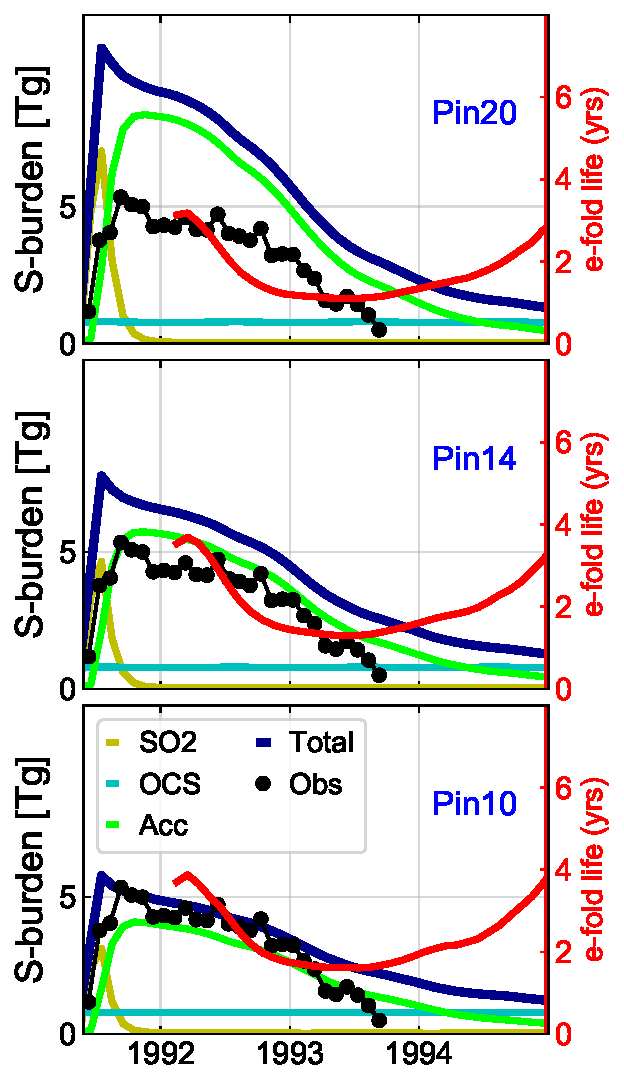
\includegraphics[width=.6\textwidth,height=.8\textheight,trim={0.1cm 0.1cm 0.1cm 0.1cm},clip]{Pin_burden.pdf}
\caption{Global stratospheric (above 8 km) Sulphur burden (S-burden, black line)}
% in Tg 
%in \Pin10 (top), \Pin14 (middle) and \Pin20 (bottom) simulations.
%Partial S-burden contribution from  SO$_2$,  OCS and Accumulation mode  is shown with 
%yellow, cyan and green lines, respectively. 
%Estimated e-folding time (calculated using $\pm$ 6 month total burden values) is also shown with red lines.}
\label{fig:pburden}
\end{figure}




\newpage
\begin{figure}[ht!]
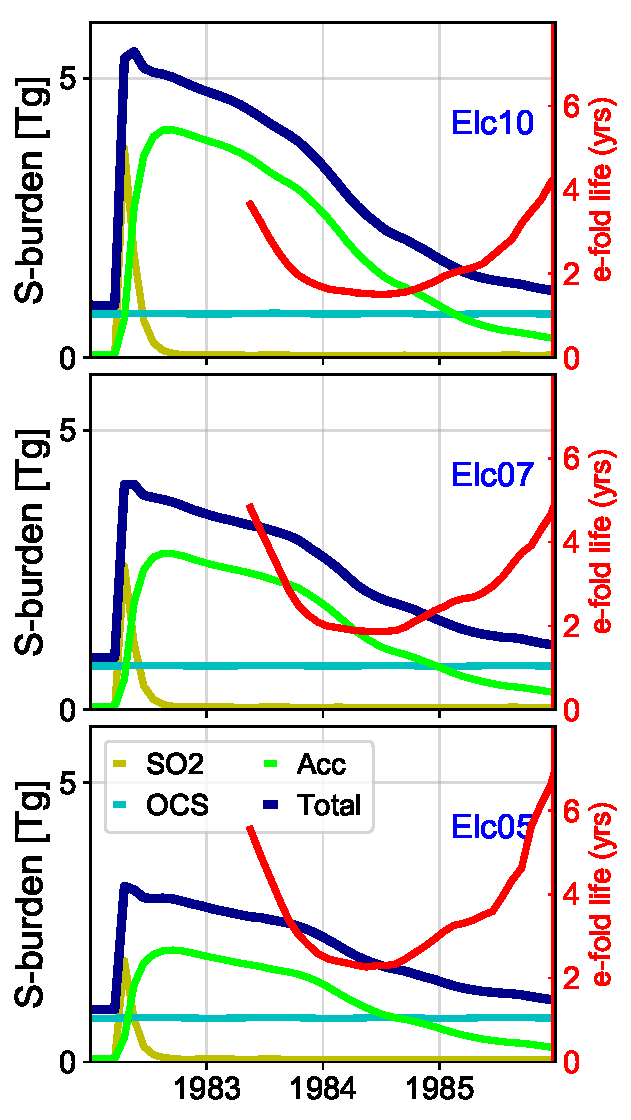
\includegraphics[width=.6\textwidth,height=.8\textheight,trim={0.1cm 0.1cm 0.1cm 0.1cm},clip]{Elc_burden.pdf}
\caption{Same as ~\ref{fig:pburden}, but for El-Chichon eruption.} 
\label{fig:eburden}
\end{figure}




\newpage
\begin{figure}[ht!]
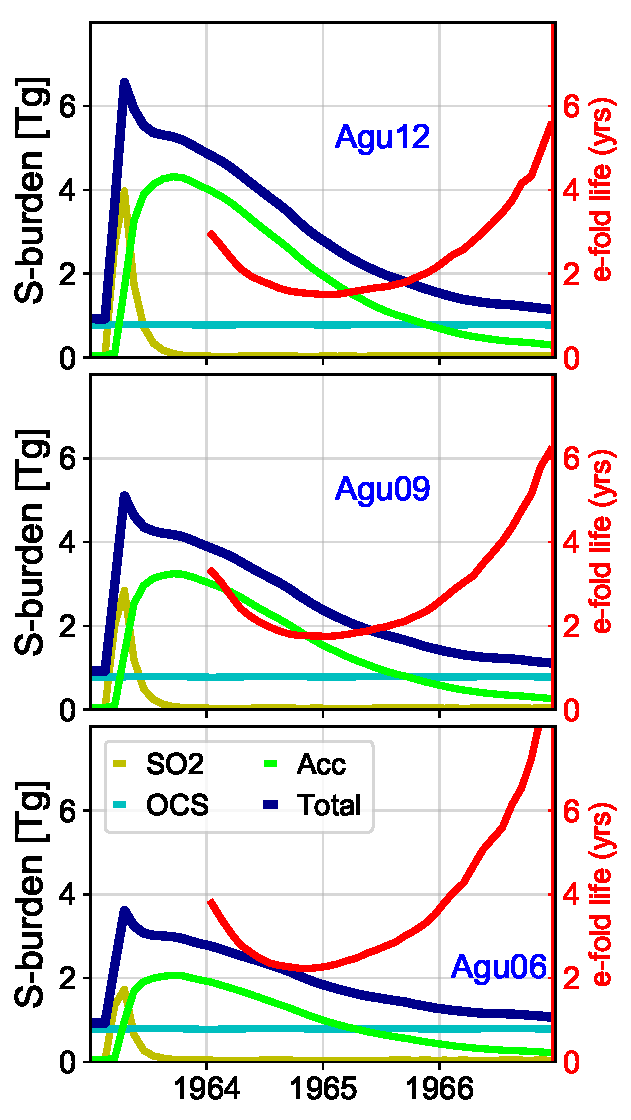
\includegraphics[width=.6\textwidth,height=.8\textheight,trim={0.1cm 0.1cm 0.1cm 0.1cm},clip]{Agu_burden.pdf}
\caption{Same as ~\ref{fig:pburden}, but for Agung eruption.} 
\label{fig:aburden}
\end{figure}





\newpage
\begin{figure}[ht!]
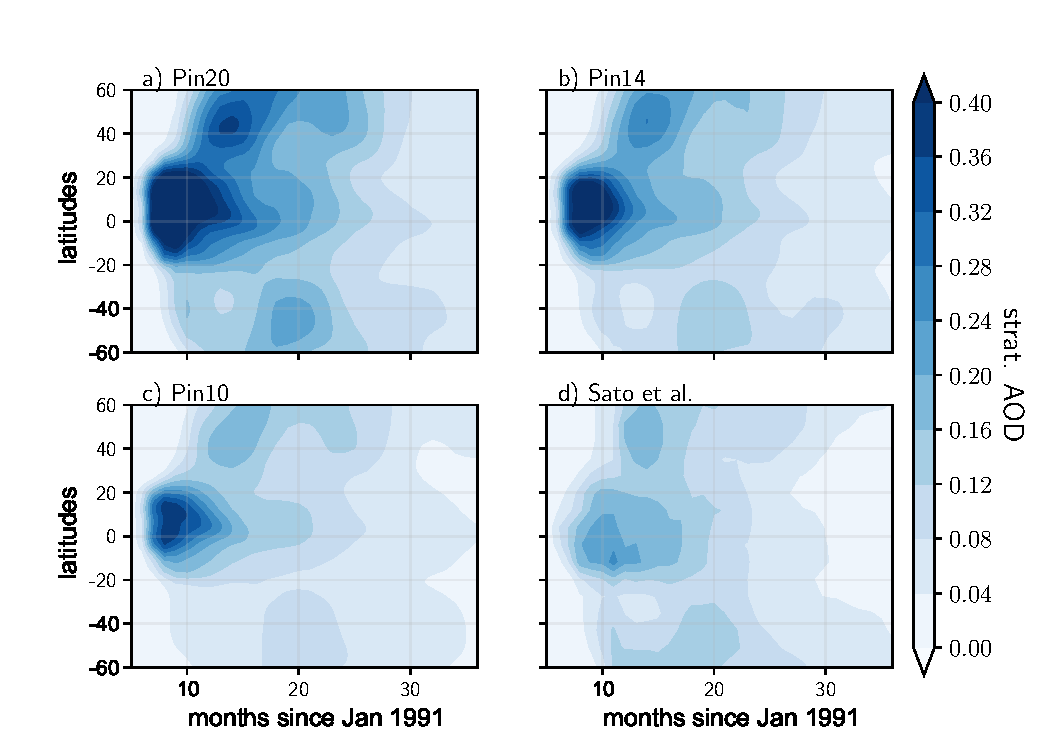
\includegraphics[width=.8\textwidth,height=.6\textheight,trim={0.1cm 0.1cm 0.1cm 0.1cm},clip]{Pin_mean_saod.pdf}
\caption{Ensemble mean stratospheric AOD (s-AOD) from \textbf{Pin20},~\textbf{Pin14}, and \textbf{Pin10} simulations.} 
\label{fig:paod}
\end{figure}

\newpage
\begin{figure}[ht!]
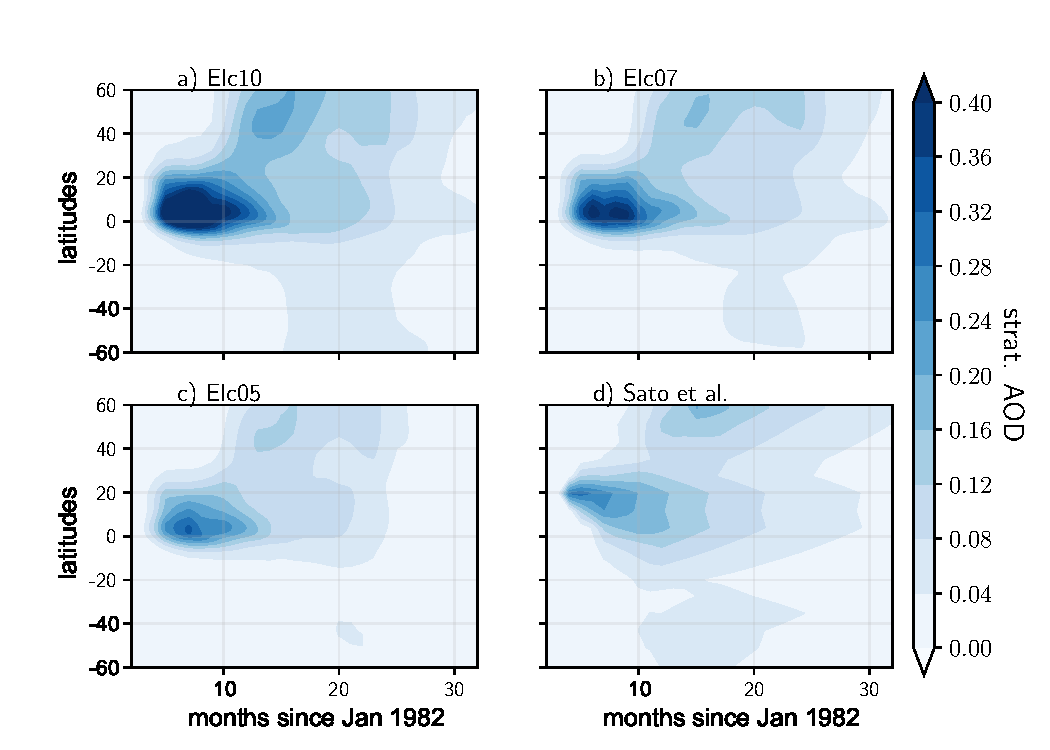
\includegraphics[width=.8\textwidth,height=.6\textheight,trim={0.1cm 0.1cm 0.1cm 0.1cm},clip]{Elc_mean_saod.pdf}
\caption{Same as ~\ref{fig:paod}, but for from \textbf{Elc10},~\textbf{Elc07}, and \textbf{Elc05} simulations.} 
\label{fig:eaod}
\end{figure}


\newpage
\begin{figure}[ht!]
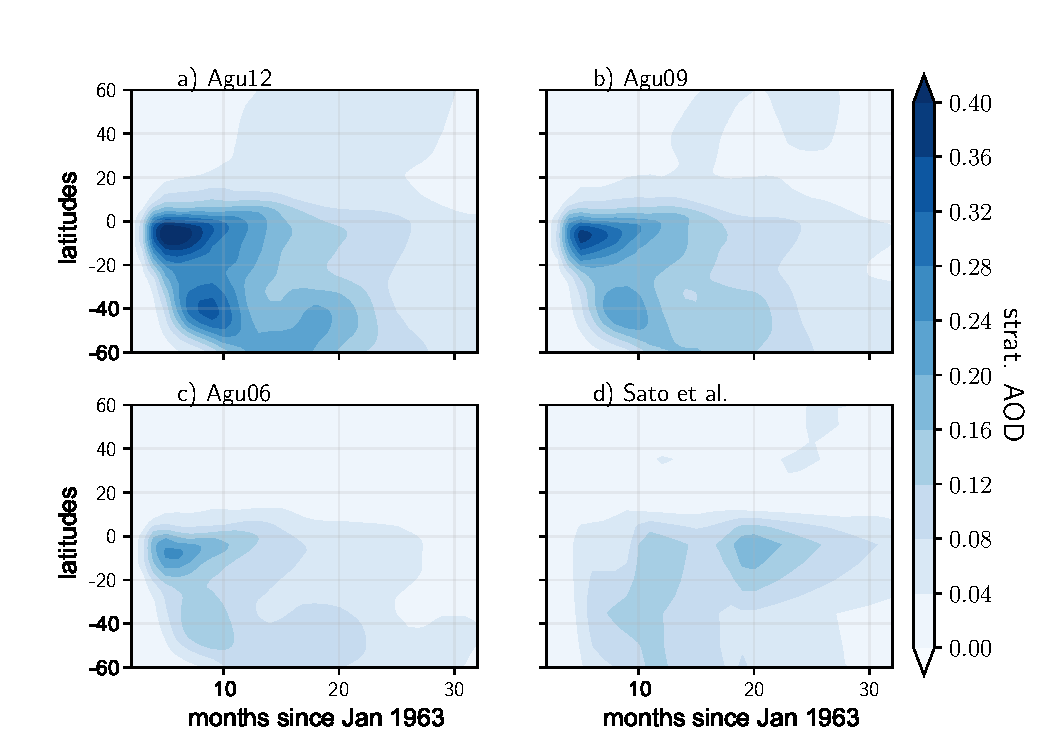
\includegraphics[width=.8\textwidth,height=.6\textheight,trim={0.1cm 0.1cm 0.1cm 0.1cm},clip]{Agu_mean_saod.pdf}
\caption{Same as ~\ref{fig:paod}, but for from \textbf{Agu12},~\textbf{Agu09}, and \textbf{Agu06} simulations.} 
\label{fig:aaod}
\end{figure}




\newpage
\begin{figure}[ht!]
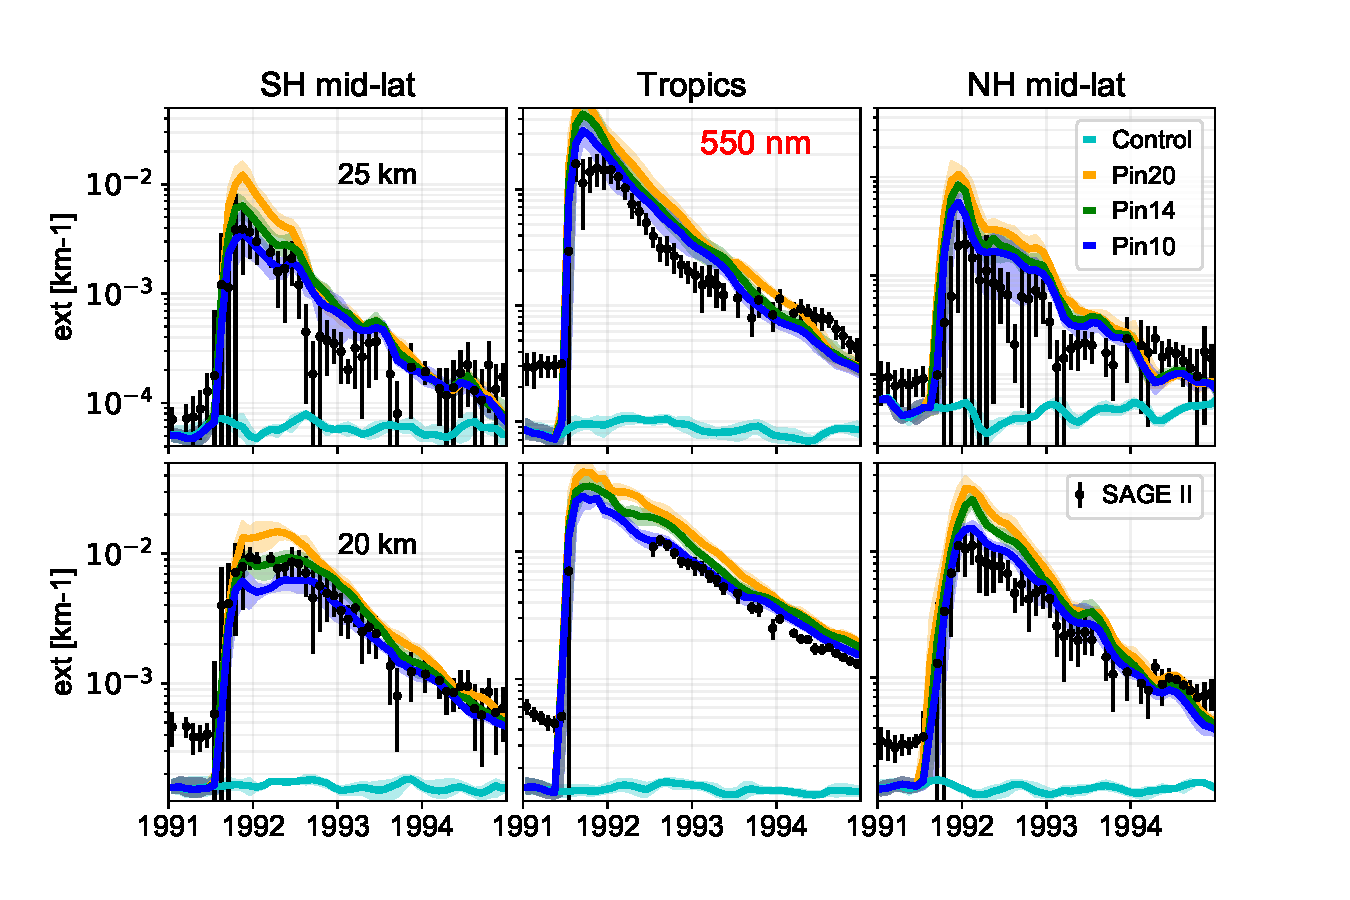
\includegraphics[width=1.0\textwidth,height=.6\textheight,trim={0.1cm 0.1cm 0.1cm 0.1cm},clip]{Pinatubo_ext_550.pdf}
\caption{Ensemble mean extinctions (550~nm) at 25~km (top) and 20~km (bottom) from \textbf{Control} (aqua), \textbf{Pin20} (orange), \textbf{Pin14} (green), and \textbf{Pin10} (blue) simulations. Shaded region shows variability among ensemble members. Extinctions for SH mid-latitudes (35\si{\degree}S -- 60\si{\degree}S), tropics (20\si{\degree}S -- 20\si{\degree}N), and  (35\si{\degree}S -- 60\si{\degree}S) are shown in left, middle and right panels, respectively. Monthly mean extiction from SAGE II v7.2 mesurments for a given latitude band are shown with black filled circles and vertical lines indicate standard deviation from all the mesurements for a given month. }
\label{fig:pext}
\end{figure}





\newpage
\begin{figure}[ht!]
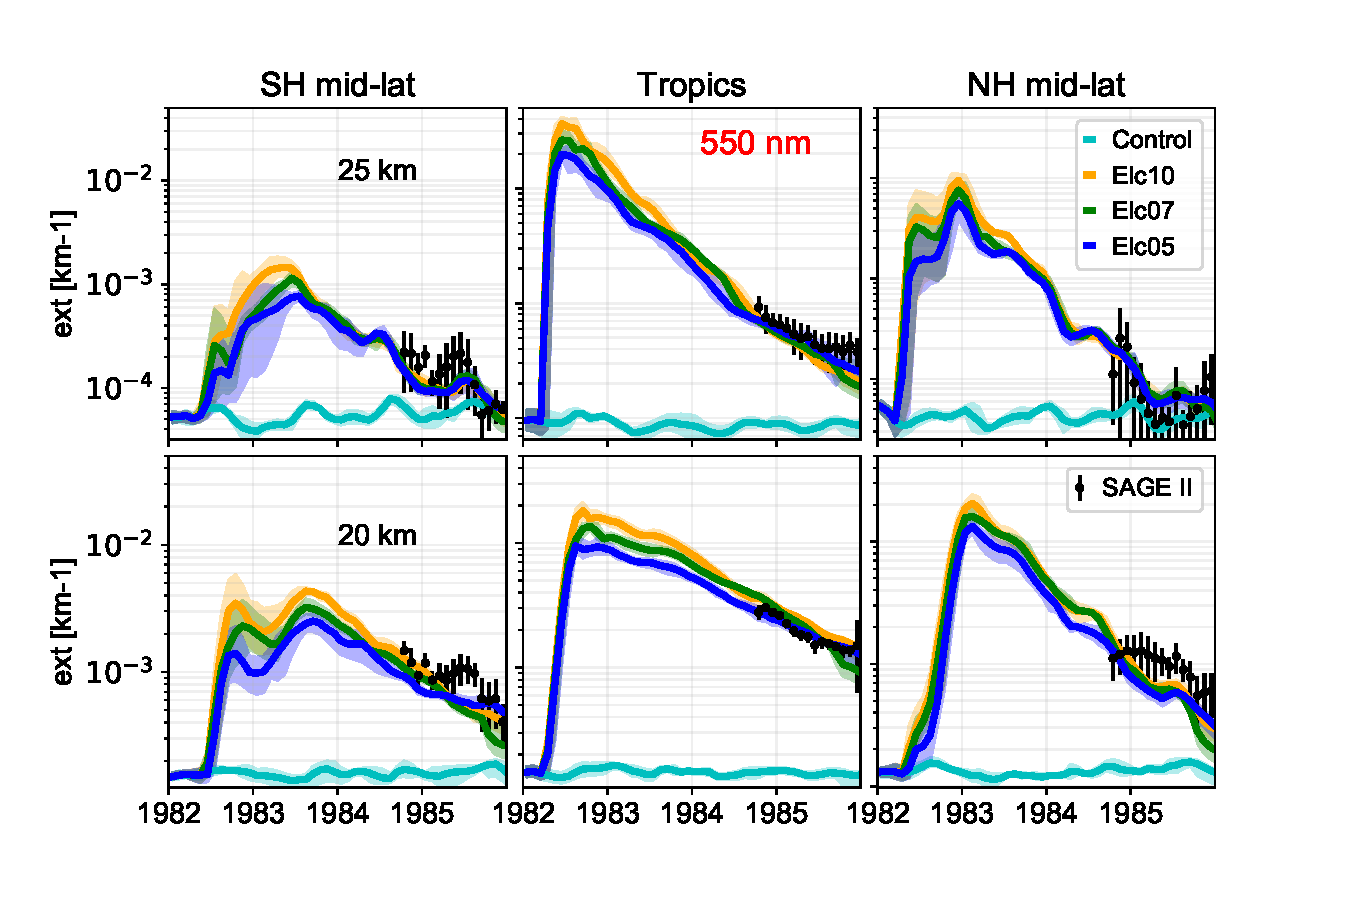
\includegraphics[width=1.0\textwidth,height=.6\textheight,trim={0.1cm 0.1cm 0.1cm 0.1cm},clip]{Elchichon_ext_550.pdf}
\caption{Same as ~\ref{fig:pext}, but for Elchichon eruption.} 
\label{fig:eext}
\end{figure}




\newpage
\begin{figure}[ht!]
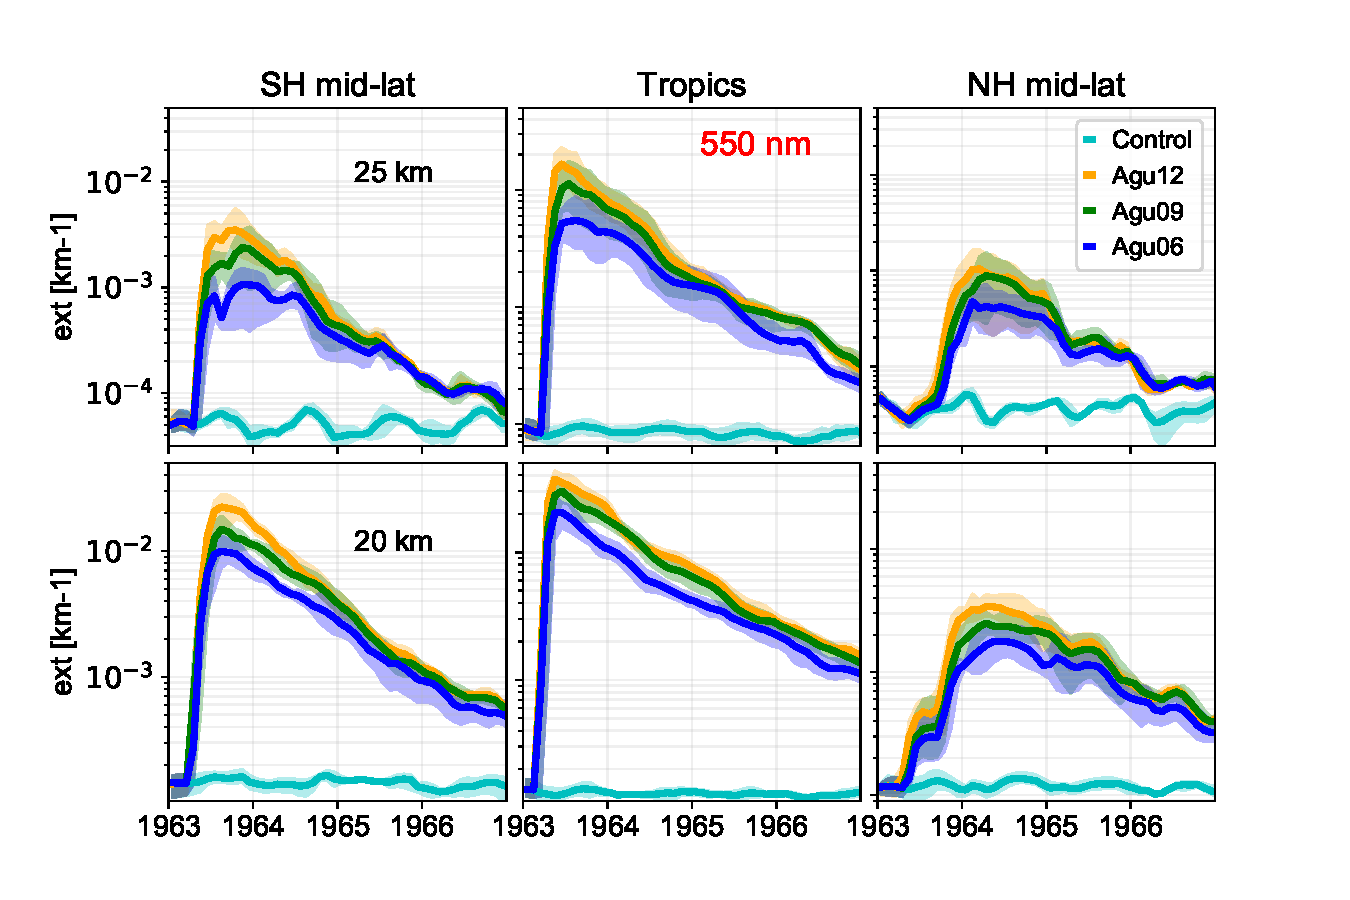
\includegraphics[width=1.0\textwidth,height=.6\textheight,trim={0.1cm 0.1cm 0.1cm 0.1cm},clip]{Agung_ext_550.pdf}
\caption{Same as ~\ref{fig:pext}, but for Agung eruption.} 
\label{fig:aext}
\end{figure}







\newpage
\begin{figure}[ht!]
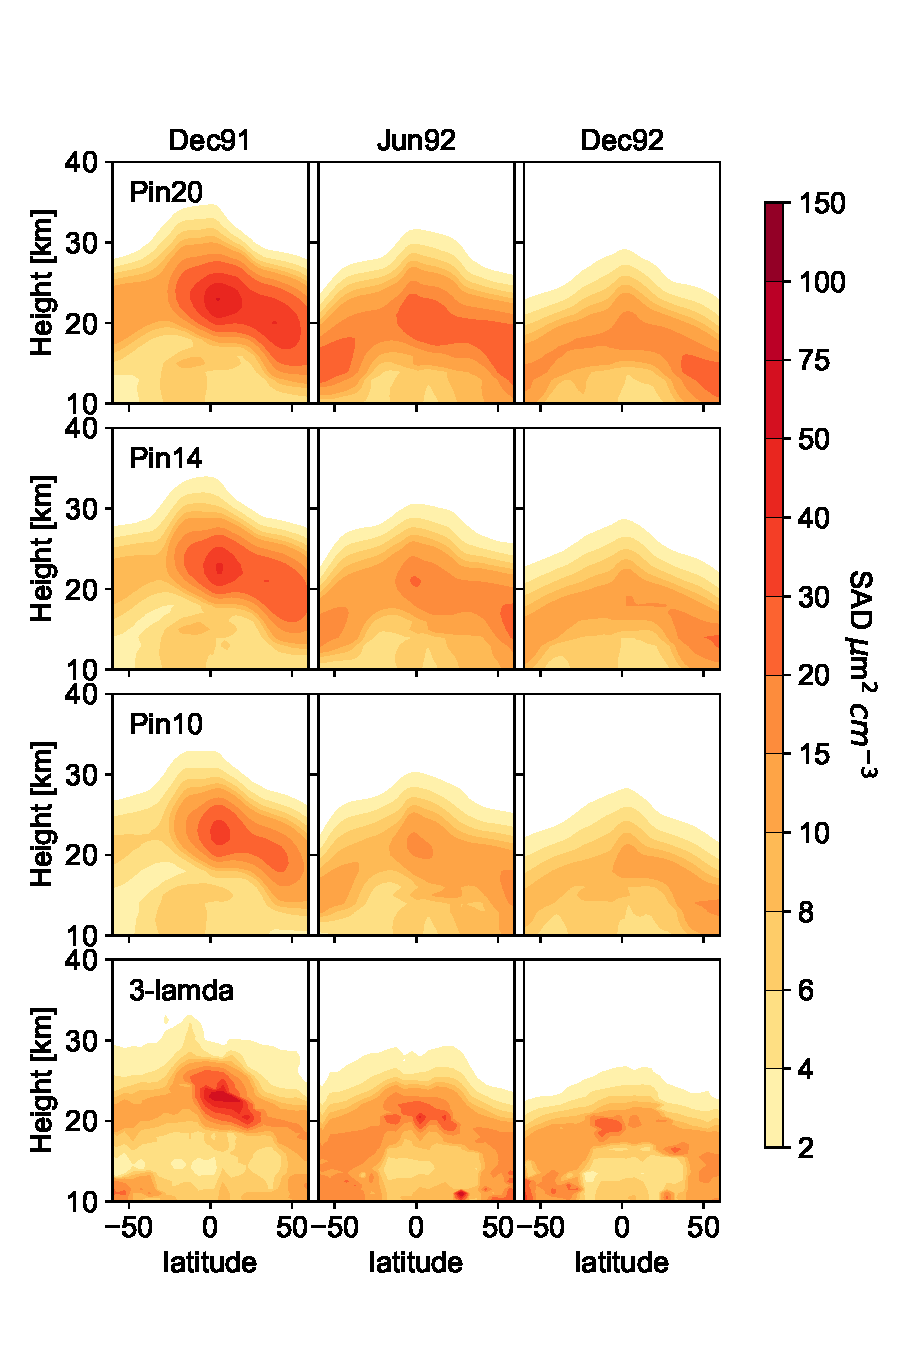
\includegraphics[width=.8\textwidth,height=.9\textheight,trim={0.1cm 0.1cm 0.1cm 0.1cm},clip]{Pin_sad.pdf}
\caption{Zonal mean monthly mean Sulphate Area Density (SAD, \unit{{\mu}m^2\,cm^{-3\xspace}}) from
 (top) \textbf{Pin20},~(second) \textbf{Pin14}, and (third)~\textbf{Pin10} model simulations.
 Bottom panel shows SAD derived using various satellite and in-situ measurements \citet{Arfeuille2013\xspace}}
\label{fig:psad}
\end{figure}

\newpage
\begin{figure}[ht!]
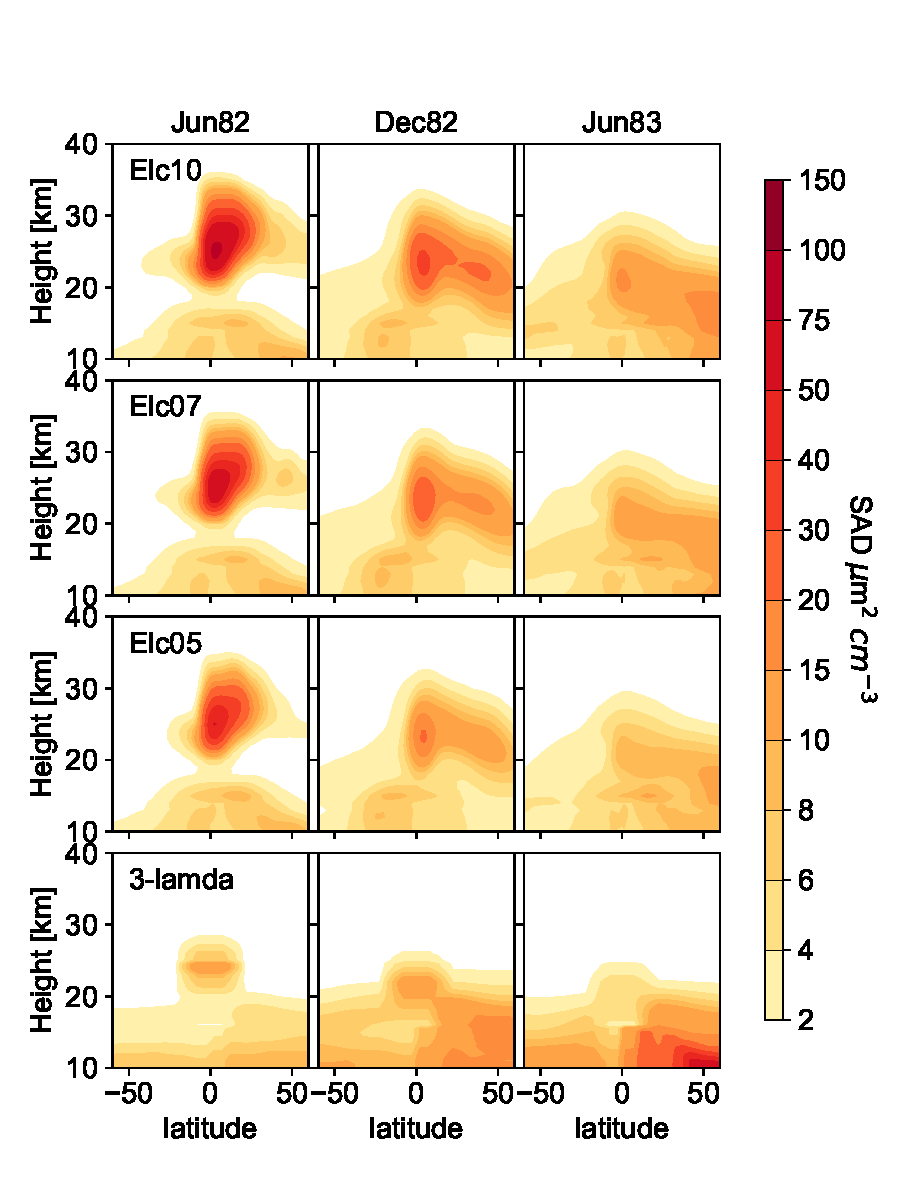
\includegraphics[width=.8\textwidth,height=.9\textheight,trim={0.1cm 0.1cm 0.1cm 0.1cm},clip]{Elc_sad.pdf}
\caption{Same as ~\ref{fig:psad}, but for El-Chichon eruption.} 
\label{fig:esad}
\end{figure}


\newpage
\begin{figure}[ht!]
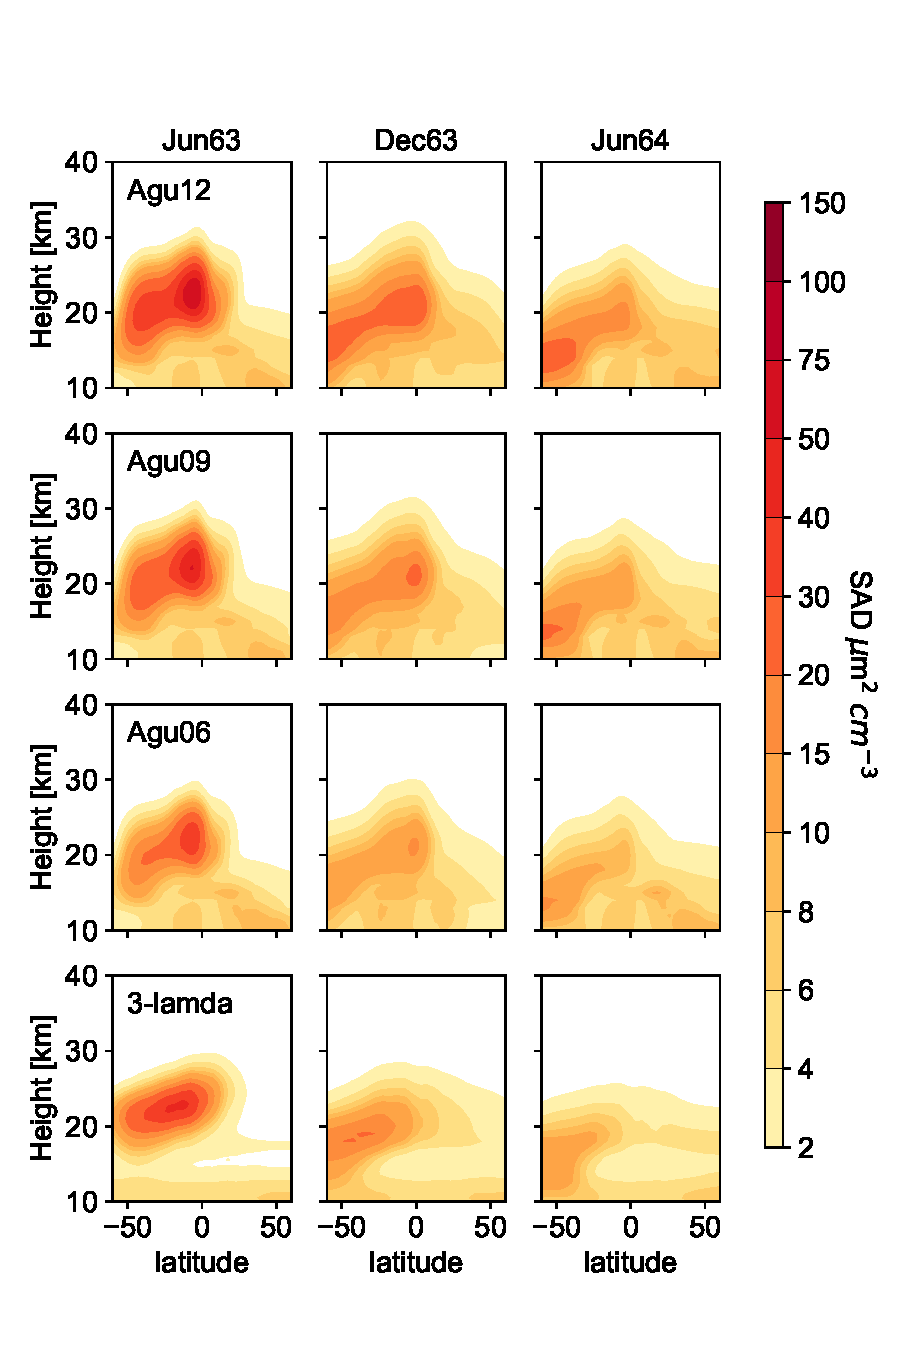
\includegraphics[width=.8\textwidth,height=.9\textheight,trim={0.1cm 0.1cm 0.1cm 0.1cm},clip]{Agu_sad.pdf}
\caption{Same as ~\ref{fig:psad}, but for El-Chichon eruption.} 
\label{fig:asad}
\end{figure}


\newpage
\begin{figure}[ht!]
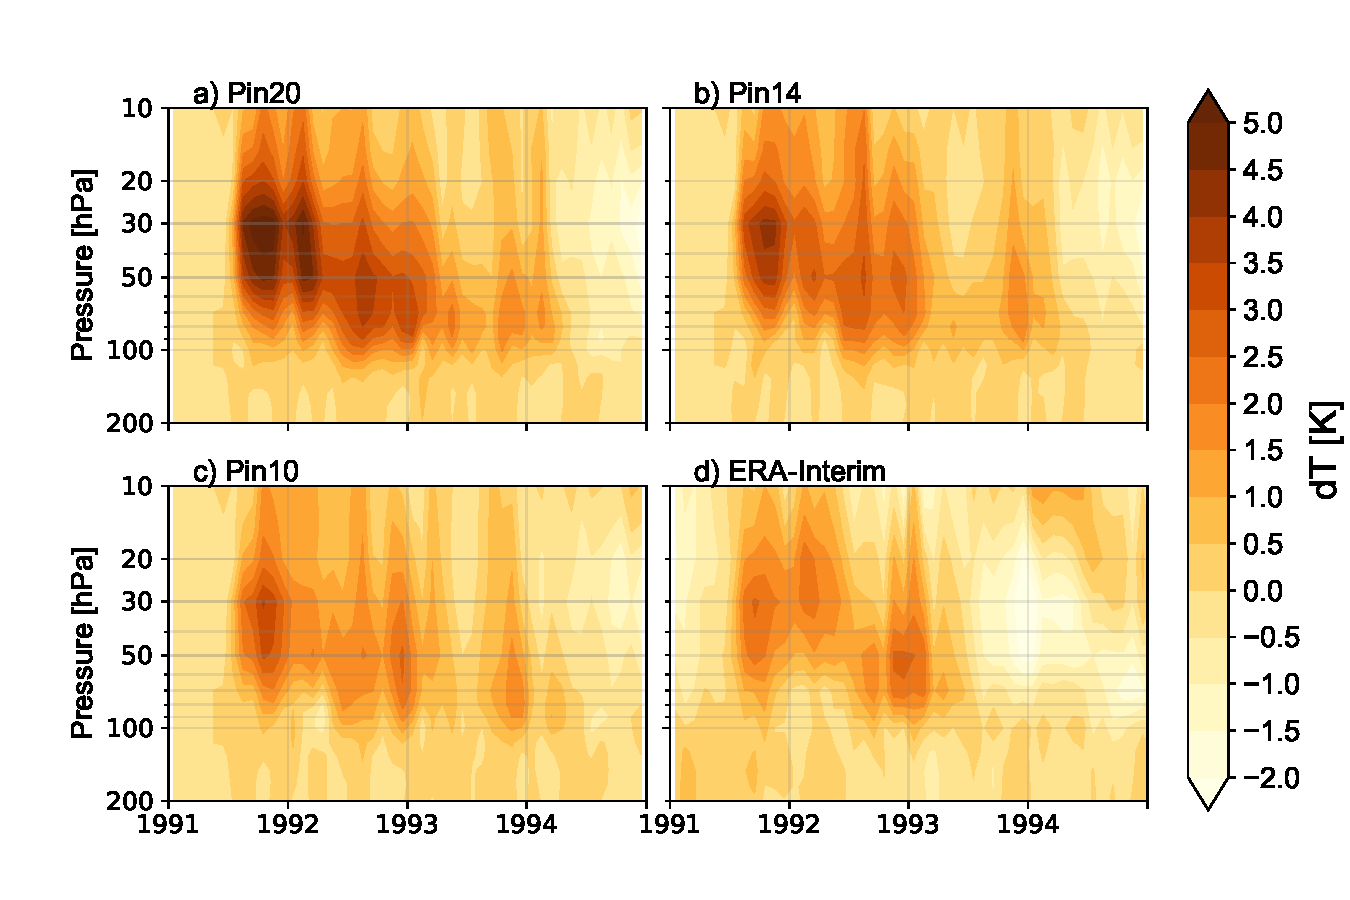
\includegraphics[width=.8\textwidth,height=.6\textheight,trim={0.1cm 0.1cm 0.1cm 0.1cm},clip]{Pinatubo_dt.pdf}
\caption{Aerosol induced heating in the tropical stratosphere 
(20\si{\degree}S -- 20\si{\degree}N) in  \textbf{Pin20},
~\textbf{Pin14}, and ~\textbf{Pin10} simulations, 
calculated by substracting temperature fields from 
a control simulation.
 Temperature anomalies in ERA-int renalysis data (for 1991--1995 time period) 
are also shown.}
\label{fig:ptemp}
\end{figure}


\newpage
\begin{figure}[ht!]
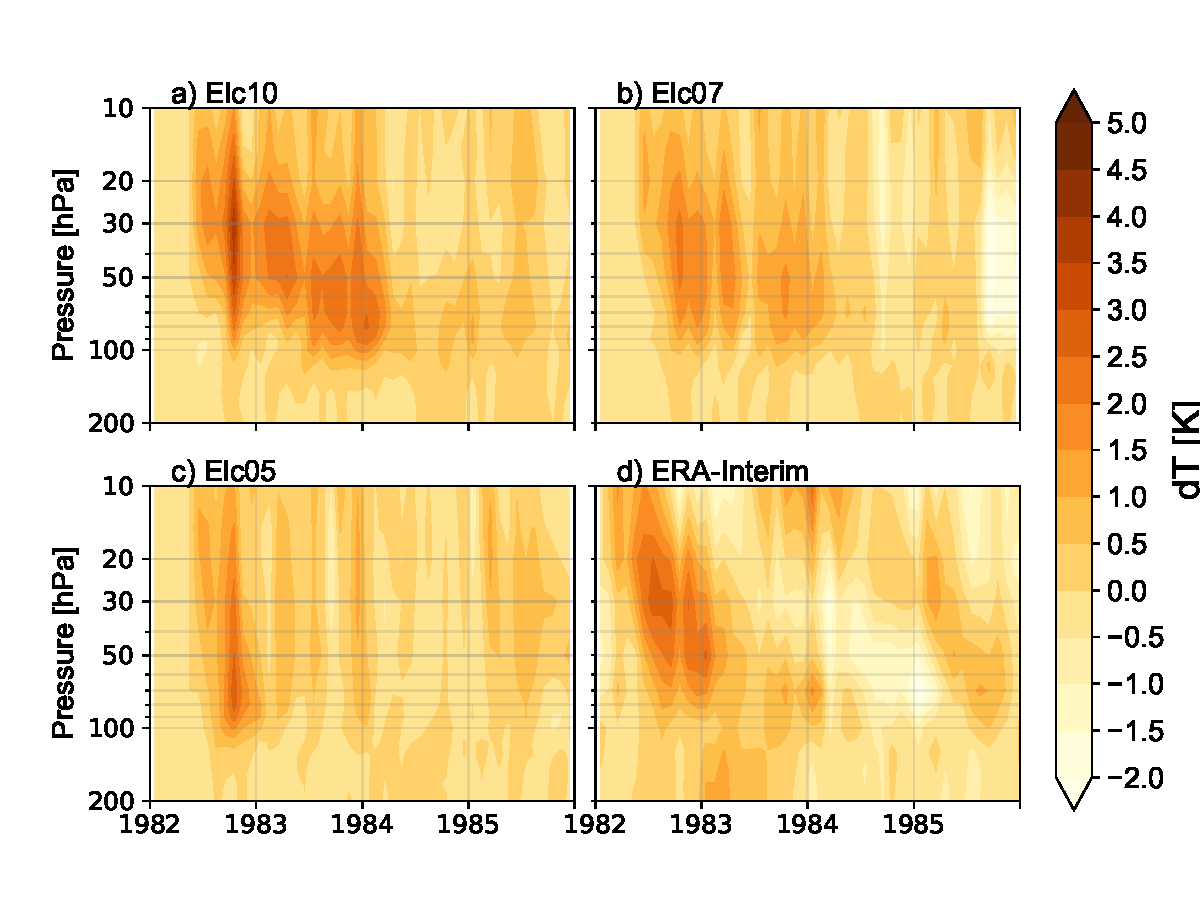
\includegraphics[width=.8\textwidth,height=.6\textheight,trim={0.1cm 0.1cm 0.1cm 0.1cm},clip]{Elchichon_dt.pdf}
\caption{Same as ~\ref{fig:ptemp}, but for El-Chichon eruption.} 
\label{fig:etemp}
\end{figure}



\newpage
\begin{figure}[ht!]
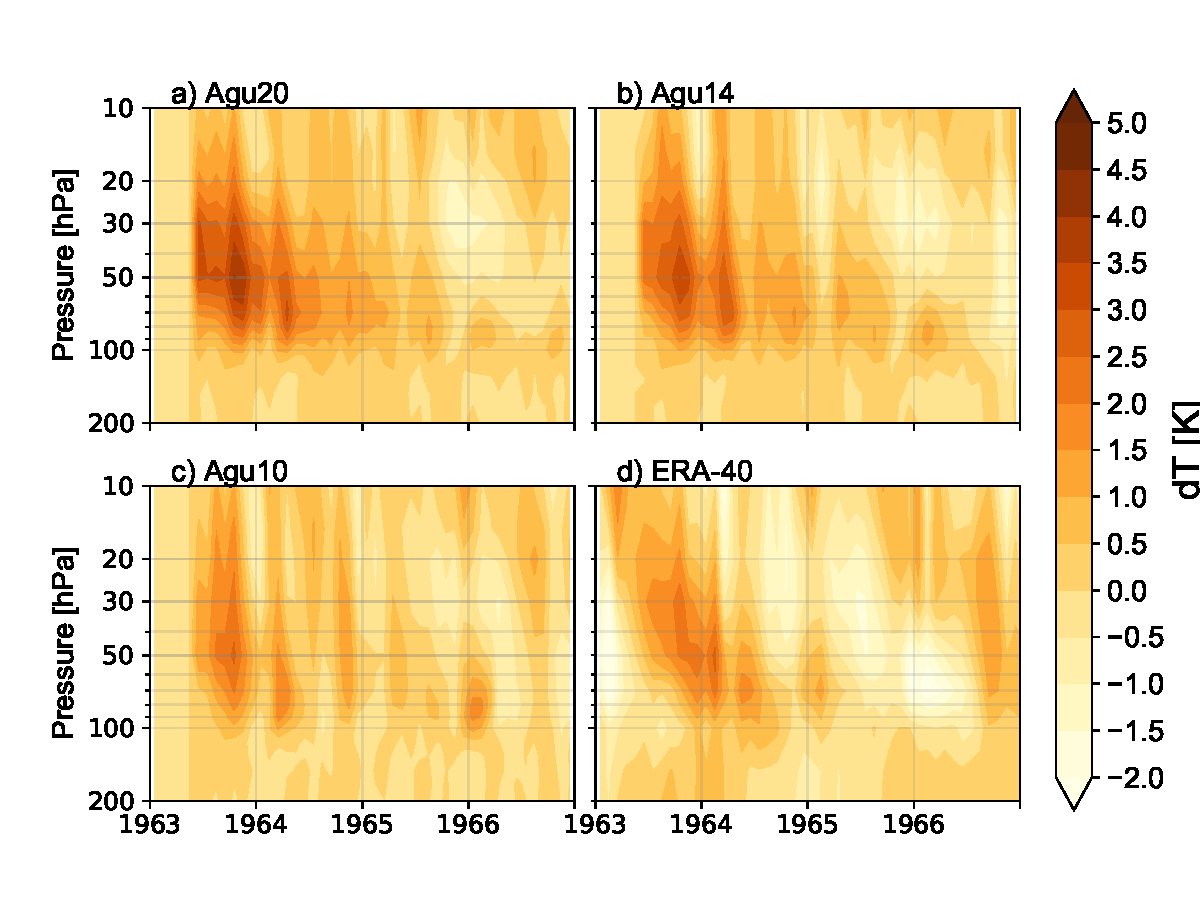
\includegraphics[width=.8\textwidth,height=.6\textheight,trim={0.1cm 0.1cm 0.1cm 0.1cm},clip]{Agung_dt.pdf}
\caption{Same as ~\ref{fig:atemp}, but for Agung eruption.} 
\label{fig:atemp}
\end{figure}


\begin{acknowledgements}
  We would  like to  thank P.~B.~Russell for effective  radius data.
  This  work was  supported  by the  UK  Natural Environment  Research
  Council  (NERC grants  NE/E005659/1 and  NE/E017150/1). GWM  and KSC
  received funding  from the National Centre  for Atmospheric Science,
  one of the  NERC research centres. GWM received  EU funding from the
  European  Research Council (ERC)  under Seventh  Framework Programme
  (FP7) consortium projects MACC  and MACC-II (grant agreements 218793
  and 283576  respectively).  CEJ, FOC were supported  as part
  the  UK Integrated Climate  Programme funded  by the  Department for
  Energy and Climate Change (DECC) and Department for Environment Food
  and Rural  Affairs --  DECC/Defra (GA01101). 
  We  would also  like to
  thank  James  Keeble for  his  help  during  model development.   We
  acknowledge  use  of the  MONSooN  system, a~collaborative  facility
  supplied  under the  Joint Weather  and Climate  Research Programme,
  which is a~strategic  partnership between the UK Met  Office and the
  Natural  Environment  Research Council.   This  work  has been  also
  supported by  NIWA as part  of its Government-funded,  core research
  programme.   The  in situ  measurements  were  supported  by the  US
  National  Science Foundation.   Current  measurements are  supported
  under grant number ATM-0437406.\hack{\\}
\hack{\\}
\end{acknowledgements}

\bibliographystyle{egu}
\bibliography{/nfs/see-fs-02_users/fbsssdh/Documents/library}

\end{document}
